\documentclass{article}

\usepackage[margin=1in]{geometry}   
\usepackage{graphicx}
\usepackage{caption}
\usepackage{subcaption}

\graphicspath{{diagrams/}}

\title{Overview TT\&C/Antenna Module}
\author{Bruno C. Messias}
\date{}

\begin{document}

\maketitle

\section{Requisitos Fundamentais}

\begin{itemize}
    \item Implementar toda a comunicação do satélite com a Ground Station via RF:
    \begin{itemize}
        \item Envio de telemetrias das baterias periódicamente;
        \item Envio de dados de altitude do ADCS via telecomando;
        \item Envio das imagens adquiridas via telecomando;
    \end{itemize}
    \item Receber telecomandos da GroundStation, como o deploy da antena;
\end{itemize}

\section{Comunicações/interfaces a serem utilizadas:}

\begin{itemize}
    \item \textbf{1xSPI:} Comunicação com o CM3+ para o envio dos pacotes de dados, e a recepção dos comandos;
    \item \textbf{6XGPIO:}
        \begin{itemize}
            \item \textbf{4xGPIO:} Para o controle do Rádio principal;
            \item \textbf{2xGPIO:} Para o controle do deploy da Antena.
        \end{itemize}
\end{itemize}

Na figura~\ref{datapath} pode ser observado as comunicações entre os módulos e na Figura~\ref{signals} os sinais de controle necessários. 

\begin{figure}[htbp]
    \centering
    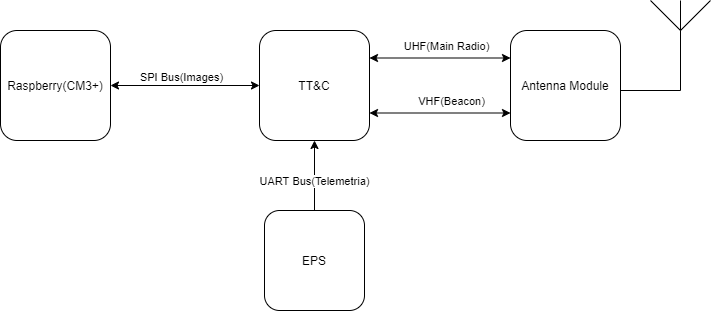
\includegraphics[scale=.5]{Datapath.png}
    \caption{Datapath Diagram}
    \label{datapath}
\end{figure}

\begin{figure}[htbp]
    \centering
    \includegraphics[scale=.5]{Control_signals.png}
    \caption{Control Signals Diagram}
    \label{signals}
\end{figure}

\section{Componente a ser utilizado:}

Será utilizado o módulo \textit{RF4463F30} interno à TT\&C com as seguintes características:

\begin{itemize}
    \item \textbf{Frequência de Operação:} 437MHz - 438MHz;
    \item \textbf{Protocolo de comunicação:} NGHam protocol;
    \item \textbf{Modulação dos Dados:} GFSK(BT= 0.5).

\end{itemize}

\section{Alimentações:}

\begin{itemize}
    \item \textbf{EPS/TTC:} 3.3V/1A, para o Rádio como alimentação padrão;
    \item \textbf{EPS/TTC:} 5V/5A, necessário quando houver uma transmissão;
    \item \textbf{EPS/Antenna:} 3.3V/2A para o deploy da Antena.
\end{itemize}

Um diagrama com as conexões de alimentação pode ser observada na Figura~\ref{power}.

\begin{figure}[htbp]
    \centering
    \includegraphics[scale=.5]{Power_buses.png}
    \caption{Power Buses Diagram}
    \label{power}
\end{figure}


\end{document}